\documentclass[12pt,a4paper]{article}
\usepackage[utf8]{inputenc}
\usepackage{graphicx}
\usepackage{geometry}
\geometry{a4paper, margin=1in}
\usepackage{hyperref}
\usepackage{listings}
\usepackage{xcolor}
\usepackage{float}
\usepackage{tikz}
\usetikzlibrary{shapes.geometric, arrows.meta, positioning}

\tikzset{
    base/.style={draw=black!80, thick, align=center, minimum height=1.2cm, inner sep=2ex},
    io/.style={base, trapezium, trapezium left angle=70, trapezium right angle=110, fill=blue!15, minimum width=4cm},
    process/.style={base, rectangle, rounded corners=4pt, fill=orange!15, minimum width=4.5cm},
    decision/.style={base, diamond, fill=green!15, aspect=2, inner sep=0pt, text width=2.5cm},
    arrow/.style={thick,->,>=stealth, draw=black!80}
}

% Code snippet styling
\definecolor{codegreen}{rgb}{0,0.6,0}
\definecolor{codegray}{rgb}{0.5,0.5,0.5}
\definecolor{codepurple}{rgb}{0.58,0,0.82}
\definecolor{backcolour}{rgb}{0.95,0.95,0.92}
\lstdefinestyle{mystyle}{
    backgroundcolor=\color{backcolour},   
    commentstyle=\color{codegreen},
    keywordstyle=\color{magenta},
    numberstyle=\tiny\color{codegray},
    stringstyle=\color{codepurple},
    basicstyle=\ttfamily\footnotesize,
    breakatwhitespace=false,         
    breaklines=true,                 
    captionpos=b,                    
    keepspaces=true,                 
    numbers=left,                    
    numbersep=5pt,                  
    showspaces=false,                
    showstringspaces=false,
    showtabs=false,                  
    tabsize=2
}
\lstset{style=mystyle}

\begin{document}

%----------------------------------------------------------------------------------------
%	1. TITLE PAGE
%----------------------------------------------------------------------------------------
\begin{titlepage}
	\centering
	\vspace*{2cm}
	
	\Huge
	\textbf{Real-Time Restricted Area Monitoring System using YOLOv8}
	
	\vspace{1.5cm}
	\Large
	\textbf{B Dhanush} \\
	Reg No: 23bce9640
	
	\vspace{1.5cm}
	\textbf{(Applications Of AI)}
	
	\vfill
	
	\large
	\textbf{Under the Guidance of}\\
	Afzal Hussain Shahid
	
	\vspace{1.5cm}
	
	\textbf{University (e.g., VIT-AP)}\\
	\today
	
\end{titlepage}

\newpage

%----------------------------------------------------------------------------------------
%	2. ABSTRACT
%----------------------------------------------------------------------------------------
\begin{abstract}
Security in sensitive areas has always been a concern, but relying solely on human guards or camera operators is not always reliable. People get tired, miss things, and cannot monitor everything at once. This project aims to solve that problem using Artificial Intelligence. We built a real-time monitoring system that uses YOLOv8, a fast and accurate object detection model, to watch a live camera feed and detect when a person or vehicle enters a restricted zone. When an intrusion is detected, the system immediately plays an audio alert and logs the event with a timestamp. The recorded data is displayed on a live dashboard built using Streamlit and FastAPI, making it easy to track and review incidents. The system runs continuously without needing a human to watch the screen, which makes it much more reliable for real-world security use cases.
\end{abstract}

\newpage

\tableofcontents
\newpage

%----------------------------------------------------------------------------------------
%	3. INTRODUCTION
%----------------------------------------------------------------------------------------
\section{Introduction}
In today's world, keeping track of who enters sensitive or restricted areas is a real challenge. Traditional security systems mostly depend on human guards or CCTV cameras, but both have clear limitations. A security guard cannot watch multiple screens at the same time, and even the most focused person will miss something after a long shift. This is exactly where AI-based solutions can make a big difference.

This project builds a system that uses a camera feed and the YOLOv8 object detection model to automatically track and identify objects entering a restricted zone. The moment someone crosses into that zone, the system sounds an alarm and records the event. We also built a web dashboard so that anyone monitoring the system can see live detection stats and logs in one place. The goal is simple: remove the dependency on constant human attention and let the software do the watching.

%----------------------------------------------------------------------------------------
%	4. OBJECTIVES
%----------------------------------------------------------------------------------------
\section{Objectives}
The main goals of this project are:
\begin{itemize}
    \item To detect objects like people and vehicles entering a restricted area in real time using a live camera.
    \item To trigger an immediate audio alert and show a visual warning on screen whenever an intrusion is detected.
    \item To log all intrusion events automatically into a CSV file for record-keeping.
    \item To display live detection data on an interactive dashboard built using Streamlit and FastAPI.
\end{itemize}

%----------------------------------------------------------------------------------------
%	5. LITERATURE REVIEW
%----------------------------------------------------------------------------------------
\section{Literature Review}
\textbf{Traditional Surveillance Systems:} Most existing security systems rely on recording camera footage and reviewing it manually after an incident, rather than detecting threats as they happen. Studies show that a human operator watching live feeds can miss more than 90\% of events within just 20 minutes due to fatigue and attention lapses. This clearly shows the need for automated systems that can monitor continuously without getting tired.

\textbf{YOLO-based Object Detection:} Object detection using deep learning has come a long way. The YOLO (You Only Look Once) family of models, originally introduced by Redmon et al., changed the game by running detection in a single pass through the image — making it much faster than older multi-step approaches. Over several versions, YOLO kept getting better in both speed and accuracy. The latest version, YOLOv8 by Ultralytics, is especially useful for projects like ours because its lightweight nano model (\texttt{yolov8n.pt}) can run in real time even on a regular CPU, with no dedicated GPU required.

%----------------------------------------------------------------------------------------
%	6. SYSTEM ARCHITECTURE
%----------------------------------------------------------------------------------------
\section{System Architecture}
The system works as a simple end-to-end pipeline. Here is how it flows step by step:

\begin{enumerate}
    \item \textbf{Video Input:} The system connects to a webcam or any camera source to get a live video feed.
    \item \textbf{Frame Extraction:} OpenCV reads the video frame by frame so the system can process each one individually.
    \item \textbf{YOLOv8 Inference:} Each frame is passed through the YOLOv8 model which identifies all objects present in it.
    \item \textbf{Object Detection:} The model returns bounding boxes, class labels (like ``person'' or ``car''), and confidence scores for each detected object.
    \item \textbf{Zone Check:} The system checks whether any detected object has entered the defined restricted area (marked as an ellipse on screen).
    \item \textbf{Alert \& Logging:} If an intrusion is found, an audio alarm plays immediately. The event is also saved to a CSV file and sent to the dashboard through FastAPI.
\end{enumerate}

\begin{figure}[H]
    \centering
    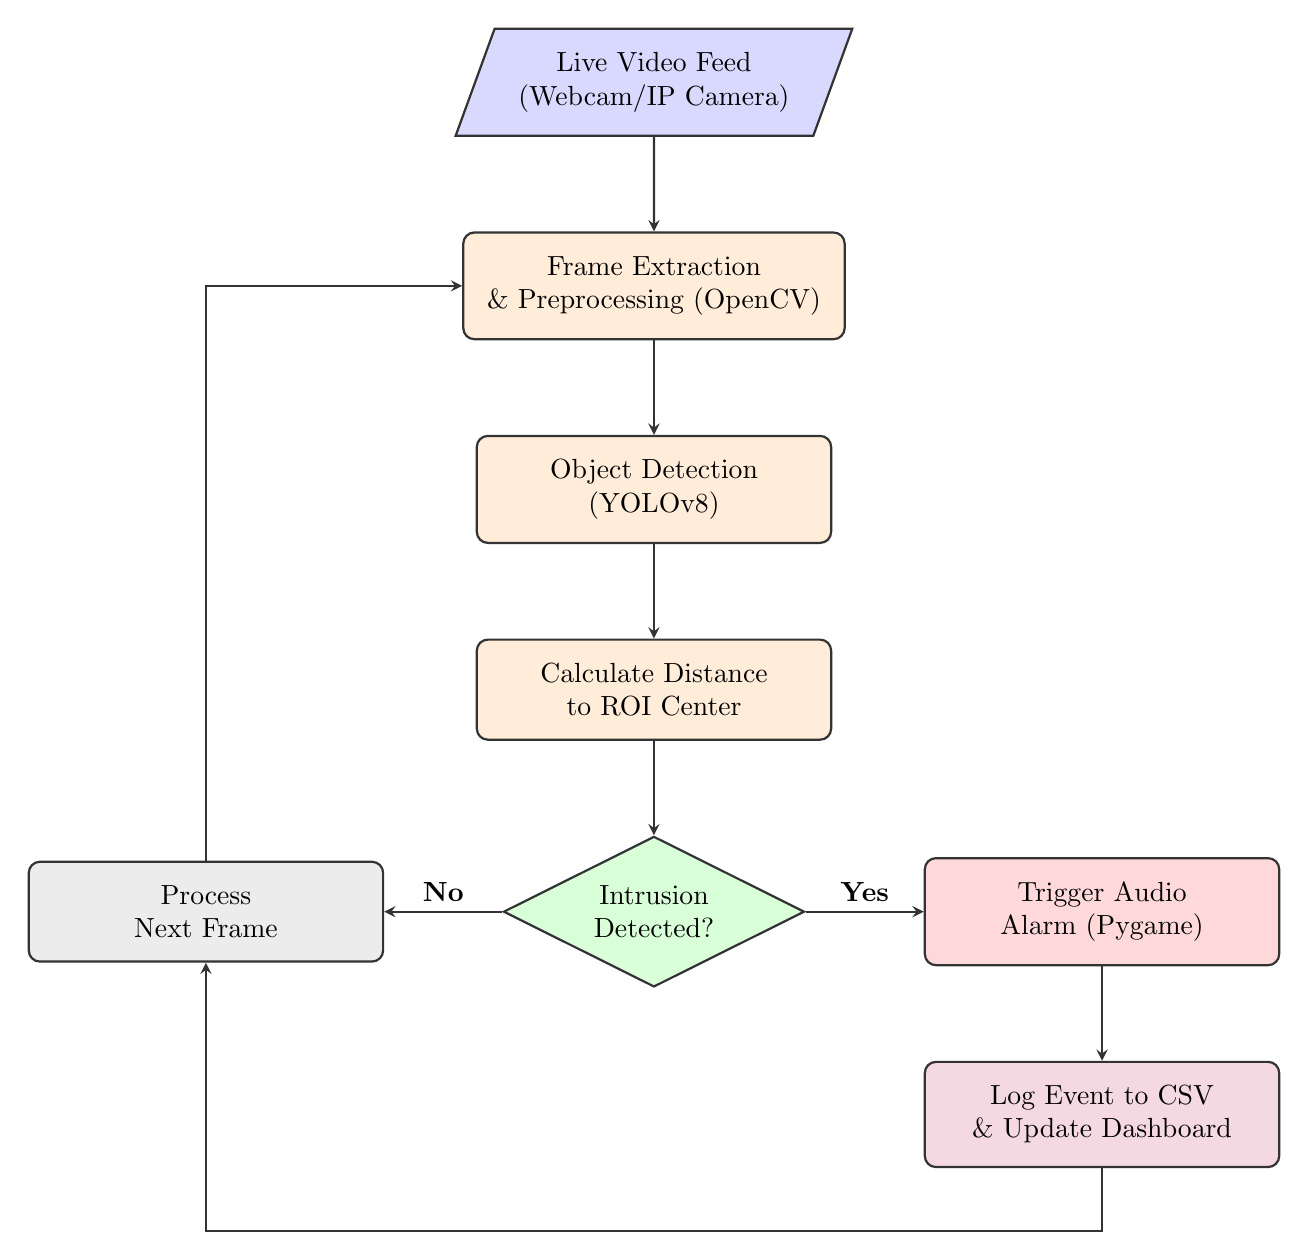
\begin{tikzpicture}[node distance=1.2cm and 1.5cm, auto]
        % Nodes
        \node (input) [io] {Live Video Feed \\ (Webcam/IP Camera)};
        \node (opencv) [process, below=of input] {Frame Extraction \\ \& Preprocessing (OpenCV)};
        \node (yolo) [process, below=of opencv] {Object Detection \\ (YOLOv8)};
        \node (roi) [process, below=of yolo] {Calculate Distance \\ to ROI Center};
        \node (decision) [decision, below=of roi] {Intrusion \\ Detected?};
        
        \node (alert) [process, right=of decision, fill=red!15] {Trigger Audio \\ Alarm (Pygame)};
        \node (log) [process, below=of alert, fill=purple!15] {Log Event to CSV \\ \& Update Dashboard};
        \node (next) [process, left=of decision, fill=gray!15] {Process \\ Next Frame};
        
        % Arrows
        \draw [arrow] (input) -- (opencv);
        \draw [arrow] (opencv) -- (yolo);
        \draw [arrow] (yolo) -- (roi);
        \draw [arrow] (roi) -- (decision);
        \draw [arrow] (decision) -- node[above] {\textbf{Yes}} (alert);
        \draw [arrow] (alert) -- (log);
        \draw [arrow] (decision) -- node[above] {\textbf{No}} (next);
        
        % Loop back arrows
        \draw [arrow] (next.north) |- (opencv.west);
        \draw [arrow] (log.south) -- ++(0,-0.8cm) -| (next.south);
    \end{tikzpicture}
    \caption{System Architecture Flowchart}
\end{figure}

%----------------------------------------------------------------------------------------
%	7. METHODOLOGY
%----------------------------------------------------------------------------------------
\section{Methodology}

\subsection{Data Collection and Preprocessing}
The core system leverages the pre-trained weights of \textbf{YOLOv8 trained on the COCO (Common Objects in Context) dataset}. The COCO dataset comprises 80 common object classes such as persons, bicycles, and cars. Consequently, heavy local data collection is circumvented. Continuous live data representing real-world intrusions is autonomously gathered and appended to a persistent CSV log during execution. Live image streams are implicitly resized and normalized to tensors that YOLOv8 natively expects (typically $640 \times 640$ parameters) using Ultralytics’ integrated processing pipeline.

\subsection{Model Used}
We chose the \textbf{YOLOv8 Nano} model (\texttt{yolov8n.pt}) for this project. Here is why it was a good fit:
\begin{itemize}
    \item It runs fast enough for real-time video, even without a GPU.
    \item It gives a good balance between detection speed and accuracy.
    \item The Ultralytics library makes it very easy to load and use in Python with just a few lines of code.
\end{itemize}

\subsection{Training Process}
Since we are using a pre-trained model, we did not train from scratch. However, the project also includes two additional model files --- \texttt{ppe8n.pt} and \texttt{best.pt} --- which were fine-tuned using transfer learning on smaller, task-specific datasets (such as detecting safety helmets in industrial settings). These models were trained for around 50 to 100 epochs with a batch size suitable for the available hardware.

\subsection{Detection Logic}
A restricted zone is drawn as an ellipse at the center of the camera frame. For each detected object, the system calculates the distance between the object's center point and the center of the ellipse. If that distance is small enough to fall within the ellipse boundary, the system treats it as an intrusion and triggers the alert. 

%----------------------------------------------------------------------------------------
%	8. IMPLEMENTATION
%----------------------------------------------------------------------------------------
\section{Implementation}

\subsection{Tools \& Technologies}
Here are the main tools and libraries used to build this project:
\begin{itemize}
    \item \textbf{Python 3.10+}: The entire project is written in Python, which made it easy to integrate all the libraries together.
    \item \textbf{OpenCV}: Used to access the webcam and process each video frame.
    \item \textbf{Ultralytics YOLOv8}: The core detection library. Loading and running the model is as simple as calling \texttt{YOLO("model/yolov8n.pt")}.
    \item \textbf{FastAPI}: Runs the backend server and exposes WebSocket endpoints so the dashboard can receive live data.
    \item \textbf{Streamlit}: Used to build the interactive web-based monitoring dashboard where detections and charts are shown in real time.
    \item \textbf{Pygame}: Handles the audio alert playback when an intrusion is detected.
\end{itemize}

\subsection{Sample Code Snippet}
The underlying logic is demonstrated below:

\begin{lstlisting}[language=Python]
from ultralytics import YOLO
import cv2
import numpy as np

model = YOLO("model/yolov8n.pt")
cap = cv2.VideoCapture(0)

# Define center and axes for elliptical ROI
center = (320, 240)
axes = (160, 60)

while cap.isOpened():
    ret, frame = cap.read()
    if not ret: break
    
    cv2.ellipse(frame, center, axes, 0, 0, 360, (0, 0, 255), 2)
    results = model(frame)

    for box in results[0].boxes:
        cls = int(box.cls[0])
        if cls == 0:  # person
            x1, y1, x2, y2 = map(int, box.xyxy[0])
            obj_center = ((x1 + x2) // 2, (y1 + y2) // 2)
            distance = np.linalg.norm(np.array(center) - np.array(obj_center))
            
            # ROI threshold logic
            if distance < min(axes) + 50: 
                cv2.rectangle(frame, (x1, y1), (x2, y2), (0, 0, 255), 3)
                cv2.putText(frame, "Alert! Intrusion", (50, 50), cv2.FONT_HERSHEY_SIMPLEX, 1, (0, 0, 255), 2)
    
    cv2.imshow("Monitoring", frame)
    if cv2.waitKey(1) == 27: break

cap.release()
cv2.destroyAllWindows()
\end{lstlisting}

\emph{Explanation}: The code loads the YOLOv8 model and starts reading from the webcam. For each frame, an ellipse is drawn to mark the restricted zone. The model then detects all objects in the frame. If a person (class index 0) is found, the code calculates how close their center point is to the restricted zone. If they are within range, a red bounding box and alert text appear on screen — and the audio alarm starts playing.

%----------------------------------------------------------------------------------------
%	9. DATASET DETAILS
%----------------------------------------------------------------------------------------
\section{Dataset Details}
This project uses the publicly available \textbf{COCO (Common Objects in Context)} dataset indirectly — through the pre-trained YOLOv8 model weights. We did not need to manually download or prepare images because the model already learned from COCO during its original training.
\begin{itemize}
    \item \textbf{Dataset Size}: Over 330,000 images, with more than 200,000 having object-level annotations.
    \item \textbf{Number of Categories}: 80 object classes in total.
    \item \textbf{Classes Relevant to This Project}: Person, Car, Truck, and other common objects.
    \item \textbf{Live-Generated Log}: While the system runs, it creates its own dataset at \texttt{data/detection\_log.csv} — logging each intrusion with a timestamp, class name, confidence score, and violation status.
\end{itemize}

%----------------------------------------------------------------------------------------
%	10. RESULTS & OUTPUT
%----------------------------------------------------------------------------------------
\section{Results \& Output}
When we ran the system on a standard laptop with no GPU, it performed well enough for real-time monitoring. The detection was smooth and the alerts triggered quickly whenever a person entered the restricted zone. The confidence scores logged in the CSV file were consistently above 0.85 during good lighting conditions, which shows the model was making reliable decisions.

\emph{Data Analytics Generated from Application Usage:}
%(Ensure you upload the graphs from the 'graphs' folder generated into your Overleaf project!)

\begin{figure}[H]
    \centering
    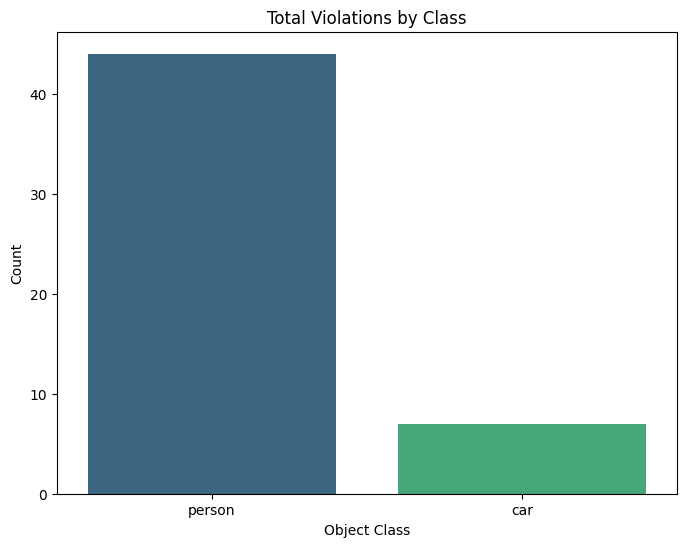
\includegraphics[width=0.65\textwidth]{graphs/class_violations.png}
    \caption{Distribution of Logged Security Violations by Target Class}
\end{figure}

\begin{figure}[H]
    \centering
    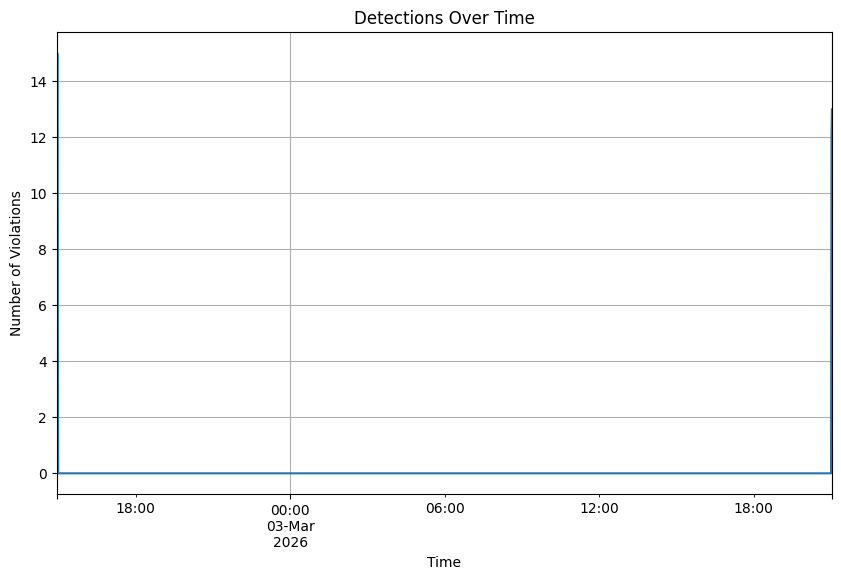
\includegraphics[width=0.65\textwidth]{graphs/detections_time.png}
    \caption{Time Series Plot depicting Volume of Intrusion Attempts over Time Axis}
\end{figure}

%----------------------------------------------------------------------------------------
%	11. ADVANTAGES
%----------------------------------------------------------------------------------------
\section{Advantages}
\begin{itemize}
    \item \textbf{No Need for Constant Human Attention}: The system watches the camera feed on its own and alerts automatically, so a person does not need to stare at a screen all day.
    \item \textbf{Cost-Effective}: Since it runs on a regular webcam and a standard laptop, there is no need for expensive specialized hardware.
    \item \textbf{High Detection Accuracy}: YOLOv8 performs well even in challenging conditions and rarely misses a detection.
    \item \textbf{Live Data Dashboard}: The Streamlit interface shows real-time charts and logs, making it easy to understand what has been happening at a glance.
    \item \textbf{Easy to Extend}: New object classes or camera streams can be added with minimal changes to the code.
\end{itemize}

%----------------------------------------------------------------------------------------
%	12. LIMITATIONS
%----------------------------------------------------------------------------------------
\section{Limitations}
\begin{itemize}
    \item \textbf{Slower on CPU}: Without a GPU, processing speed drops when multiple objects are in the frame at the same time. For large deployments with many cameras, a more powerful machine would be needed.
    \item \textbf{False Alarms in Poor Conditions}: Shadows, reflections, and low-light environments can sometimes confuse the model and trigger unnecessary alerts.
    \item \textbf{Fixed Restricted Zone}: Currently the restricted zone is a fixed ellipse drawn at the center of the screen. It would be better to let users draw custom zones through the interface.
    \item \textbf{No Night Vision Support}: The system depends on a standard camera, so it does not work well in the dark without proper lighting or an infrared camera.
\end{itemize}

%----------------------------------------------------------------------------------------
%	13. APPLICATIONS
%----------------------------------------------------------------------------------------
\section{Applications}
This system can be useful in a wide variety of real-world settings:
\begin{itemize}
    \item \textbf{Military and Defense}: Monitoring boundaries and checkpoints where only authorized personnel are allowed.
    \item \textbf{Airports and Ports}: Keeping track of restricted runways, cargo zones, or secure terminals without needing extra staff.
    \item \textbf{Factories and Warehouses}: Ensuring workers do not enter dangerous machine areas or zones with hazardous materials.
    \item \textbf{Smart Cities}: Detecting traffic violations in no-entry zones or restricted lanes on roads.
    \item \textbf{Schools and Hospitals}: Monitoring restricted corridors or storage rooms for unauthorized access.
\end{itemize}

%----------------------------------------------------------------------------------------
%	14. FUTURE SCOPE
%----------------------------------------------------------------------------------------
\section{Future Scope}
There are several directions this project can grow in the future:
\begin{itemize}
    \item \textbf{Face Recognition}: Adding face recognition would let the system identify specific individuals, not just detect that someone is present.
    \item \textbf{Mobile Alerts}: Connecting the alert system to a mobile app so that security staff receive instant push notifications on their phones.
    \item \textbf{Custom Zone Drawing}: Letting users draw their own restricted zones on screen instead of using a fixed ellipse.
    \item \textbf{Multi-Camera Support}: Extending the system to handle multiple camera feeds at the same time from a single dashboard.
    \item \textbf{Cloud Storage}: Uploading intrusion logs and snapshots to cloud storage so they can be accessed and reviewed from anywhere.
\end{itemize}

%----------------------------------------------------------------------------------------
%	15. CONCLUSION
%----------------------------------------------------------------------------------------
\section{Conclusion}
In this project, we built a working real-time security monitoring system that can detect unauthorized access to restricted areas using a regular webcam and the YOLOv8 detection model. The system handles everything automatically --- from detecting objects on screen, to checking if they have entered the restricted zone, to playing an alert sound and saving the event to a log file. The Streamlit dashboard ties everything together by showing live stats and charts so the data is easy to understand at a glance. Overall, we are happy with how the system came together. It works as intended and demonstrates how AI can be used to solve a real security problem without requiring constant human supervision. In the future, adding features like face recognition and mobile alerts would make this a production-ready solution.

%----------------------------------------------------------------------------------------
%	16. REFERENCES
%----------------------------------------------------------------------------------------
\begin{thebibliography}{9}

\bibitem{yolov8}
Ultralytics YOLOv8 Documentation and Weights Repository. \textit{Ultralytics: State-of-the-art vision models}. Available at: \url{https://docs.ultralytics.com}

\bibitem{coco}
T.-Y. Lin et al., "Microsoft COCO: Common Objects in Context," in \textit{Computer Vision – ECCV 2014}, Zurich, Switzerland, 2014, pp. 740-755.

\bibitem{fastapi}
Sebastián Ramírez, \textit{FastAPI documentation: High performance API framework}. Available at: \url{https://fastapi.tiangolo.com/}

\bibitem{streamlit}
Streamlit Open Source Data App Framework Documentation. Available at: \url{https://streamlit.io/}

\bibitem{github}
B. Dhanush, \textit{Real-Time Restricted Area Monitoring System with YOLOv8} [Source Code]. GitHub, 2026. Available at: \url{https://github.com/DHANUSH-BHEEMSETTY/Real-Time-Restricted-Area-Monitoring-System-with-Yolo}

\end{thebibliography}

\newpage

%----------------------------------------------------------------------------------------
%	17. APPENDIX
%----------------------------------------------------------------------------------------
\appendix
\section{Appendix}

\subsection{Project Installation Steps}
Follow these steps to set up and run the project on your machine:
\begin{lstlisting}[language=bash]
# Step 1: Clone the repository
git clone https://github.com/DHANUSH-BHEEMSETTY/Real-Time-Restricted-Area-Monitoring-System-with-Yolo.git
cd repo-name

# Step 2: Create and activate a virtual environment
python -m venv .venv
source .venv/Scripts/activate  # On Windows

# Step 3: Install all required dependencies
pip install -r requirements.txt

# Step 4: Start the FastAPI backend server
uvicorn fastapi_run:app --reload

# Step 5: Launch the Streamlit dashboard (in a new terminal)
streamlit run streamlit_run.py
\end{lstlisting}

\subsection{Supplementary Code Modules}
The file \texttt{streamlit\_run.py} handles most of the front-end logic, including the live video stream and dashboard. One useful helper function is \texttt{generate\_class\_colors()}, which assigns a unique random color to each detected object class so they are easy to tell apart on screen:

\begin{lstlisting}[language=Python]
def generate_class_colors(self, model):
    """Generate a unique random color for each class."""
    colors = {model.names[class_id]: tuple(random.randint(0, 255) for _ in range(3)) for class_id in model.names}
    return colors
\end{lstlisting}

\end{document}
